
    Dieser Anhang wurde am Ende des Projekts nachgereicht. Er enthält Belege für
    durchgeführte Maßnahmen, bzw. falls nicht durchgeführt eine Begründung wieso
    die Durchführung nicht möglich oder nicht erfolgt ist. \\


% ---------------------------------------------------------------------------
% statische Analysetools

\section{Statische Code-Analyse-Tools}

Um eine hohe Code-Qualität sicherzustellen und damit die Wartbarkeit der
Anwendung zu verbessern, wurden statische Analysetools eingesetzt.

\subsection{Checkstyle}

Wir haben das bekannte und beliebte Tool \glqq Checkstyle\grqq~ verwendet, um die Einhaltung von üblichen Richtlinien zum Programmierstil zu überprüfen und durchzusetzen. Diese tragen zu guter Lesbarkeit und geringer Komplexität des Quellcodes bei.

Im folgenden Abschnitt befindet sich ein Report, der erstellt wurde, als begonnen haben, \glqq Checkstyle\grqq~ einzusetzen. Anschließend haben wir alle bereits vorhandenen Warnungen in Commit 5cd67e0aff2b1edd2b42c48fd6b0a36af83a243e \glqq fixes Checkstyle warnings\grqq~ abgearbeitet. Da mit dem Plugin \glqq Checkstyle-IDEA\grqq~ alle Warnungen direkt in unserer Entwicklungsumgebung angezeigt werden, konnten diese ab dann direkt bei der Programmierung behoben werden, sodass der zweite, zum Abschluss des Projektes erstellte, Report leer ist. Ein Screenshot des Plugins mit markierten Fehlern findet sich im Abschnitt nach den Berichten.

Wir haben bei der Checkstyle-Überprüfung auf die Überprüfung verzichtet, ob Felder als private deklariert werden können, da es bei Android eine empfohlene Vorgehensweise ist, einige Felder öffentlich zu deklarieren. Dies sorgt auf mobilen Geräten für mehr Effizienz, da zum Zugreifen auf ein solches Feld keine Methode über einen Call-Stack aufgerufen werden müssen.


\includepdf[pages=1,offset=-0.8cm 0,scale=.8,pagecommand=\subsubsection{Initialer ``Checkstyle''-Report}]{anhang/partials/checkstyle-1.pdf}
\includepdf[pages=2-,offset=-0.8cm 0,scale=.8,pagecommand={}]{anhang/partials/checkstyle-1.pdf}

\includepdf[pages=1,offset=-0.8cm 0,scale=.8,pagecommand=\subsubsection{Finaler ``Checkstyle''-Report}]{anhang/partials/checkstyle-2.pdf}
\includepdf[pages=2-,offset=-0.8cm 0,scale=.8,pagecommand={}]{anhang/partials/checkstyle-2.pdf}

\subsubsection{Screenshot von Checkstyle-IDEA}

In diesem Screenshot ist sichtbar, wie Checkstyle direkt und insbesondere vor einem Commit Fehler markiert. Hier wird angemerkt, dass zwischen der Typumwandlung \glqq (Peer)\grqq~ und dem Feld \glqq other\grqq~ ein Leerzeichen fehlt, sowie dass die if-else-Konstruktion keine geschweiften Klammern verwendet.

Durch die auffällige rote Markierung kann die Checkstyle-Warnung nicht übersehen werden.

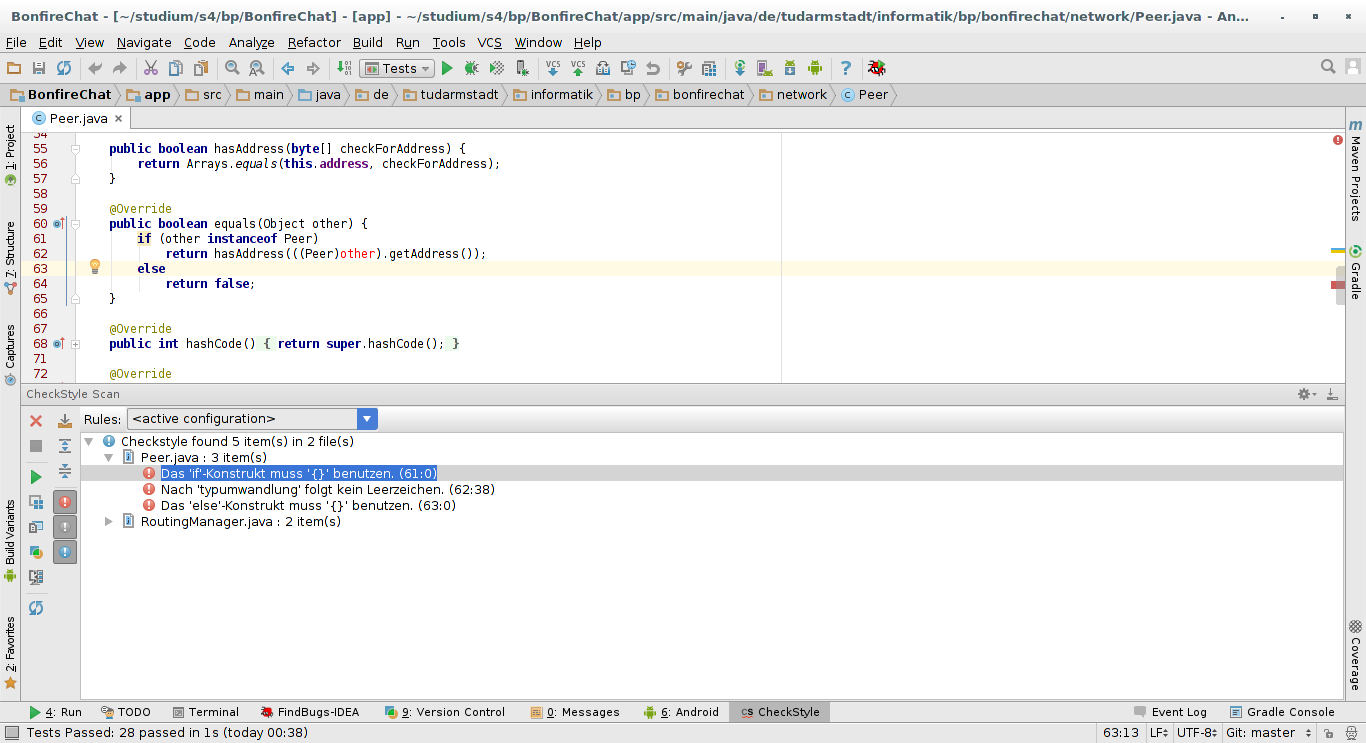
\includegraphics[width=17.5cm]{belege/checkstyle/checkstyle-idea-screenshot.png}


\clearpage
\subsection{Android Lint}

Zusätzlich haben wir das von Google entwickelte und empfohlene ``Android Lint''
genutzt. Dieses Tool gibt Empfehlungen zur Einhaltung der Android-Programmierrichtlinien.

Dadurch verbessert sich einerseits die Wartbarkeit, denn durch das Befolgen der im Android-Umfeld üblichen
 Konventionen und die Verwendung von allgemein bekannten und anerkannten Entwurfsmustern, ist der Code zukünftigen
Entwicklern leichter verständlich.
Andererseits enthalten die Reports Empfehlungen zur Verbesserung der Performance, Usability, Accessibility und Korrektheit.

Im folgenden Abschnitt befindet sich ein Report, der erstellt wurde,
als wir begonnen haben, ``Android Lint'' einzusetzen. Dann wurden initial alle
Warnungen und Empfehlungen abgearbeitet (Commit XXXXXXXXXXXXX TODO).
Die Warnungen und Empfehlungen werden direkt in der von uns verwendeten
Entwicklungsumgebung Android Studio angezeigt, sodass diese anschließend während
der Programmierung direkt umgesetzt werden konnten. Daher ist der zweite Report,
der zum Abschluss des Projekts erstellt wurde, leer.


\includepdf[pages=1,offset=-0.8cm 0,scale=.8,pagecommand=\subsubsection{Initialer ``Android Lint''-Report}]{anhang/partials/lint-results-1.pdf}
\includepdf[pages=2-,offset=-0.8cm 0,scale=.8,pagecommand={}]{anhang/partials/lint-results-1.pdf}

\includepdf[pages=1,offset=-0.8cm 0,scale=.8,pagecommand=\subsubsection{Finaler ``Android Lint''-Report}]{anhang/partials/lint-results-2.pdf}
%\includepdf[pages=2-,scale=.8,pagecommand={}]{anhang/partials/lint-results-2.pdf}


\clearpage
\subsection{FindBugs}

Um häufig auftretende Fehler zu vermeiden, haben wir FindBugs verwendet.

Im folgenden Abschnitt befindet sich ein Report, der erstellt wurde, als wir mit der Verwendung von ``FindBugs'' begonnen aben. Anschließend wurden alle Fehler und Warnungen in Commit XXXXXXXX TODO behoben. Da wir das Plugin FindBugs-IDEA direkt in unsere Entwicklungsumgebung integriert haben und Fehler so direkt markiert wurden, konnten Fehler ab dann direkt bei der Entwicklung vermieden werden und der zweite, am Ende des Projektes erstellte, Report ist leer.


\includepdf[pages=1,offset=-0.8cm 0,scale=.8,pagecommand=\subsubsection{Initialer ``FindBugs''-Report}]{anhang/partials/findbugs-1.pdf}
\includepdf[pages=2-,offset=-0.8cm 0,scale=.8,pagecommand={}]{anhang/partials/findbugs-1.pdf}

\includepdf[pages=1,offset=-0.8cm 0,scale=.8,pagecommand=\subsubsection{Finaler ``FindBugs''-Report}]{anhang/partials/findbugs-2.pdf}
\includepdf[pages=2-,offset=-0.8cm 0,scale=.8,pagecommand={}]{anhang/partials/findbugs-2.pdf}


\clearpage

% ---------------------------------------------------------------------------
% Code Reviews (Einleitung)

\section{Code Reviews}

Zur Sicherstellung der Wartbarkeit durch hohe Code-Qualität wurde bei jedem
Sprint-Treffen mit dem Auftraggeber ein Code Review durchgeführt.

% ---------------------------------------------------------------------------
% Code Reviews: Checkliste

\subsection{Checkliste}


\begin{enumerate}[ 1.]
  \item Ist die Funktionalität korrekt?
  \item Sind die Klassen, Funktionen und Variablen angemessen benannt?
  \item Wurde die Klassenstruktur gut entworfen und erfüllt sie alle Anforderungen, oder sind Verbesserungen nötig?
  \item Gibt es Klassen, die aufgrund neuer Implementierungen überflüssig geworden sind?
  \item Gibt es unnötig überladene Funktionen oder Konstruktoren?
  \item Wurde die Datenbankstruktur gut entworfen?
  \item Enthält das Codeteil Funktionen, die wiederverwendet werden können? Sind diese in einer Helper-Klasse untergebracht?
  \item Wurden existierende Helper-Funktionen benutzt? Ist keine doppelte Funktionalität implementiert?
  \item Werden alle Eingabeparameter validiert?
  \item Wie beeinflusst die Funktionalität die Performance der App - Stromverbrauch, Rechenzeit und Speicherbedarf?
  \item Ist es unbedingt nötig, den Code in einem UI-Thread laufen zu lassen oder würde ein Background-Thread ausreichen?
  \item Werden alle möglichen Fehlschläge behandelt?
  \item Findet eine ``Graceful Degradation'' statt?
  \item Werden die Best Practices zur Appentwicklung, laut Android Lint, befolgt?
  \item Welche Teile können parallel ausgeführt werden?
  \item Sind die Operationen, bei denen Threadsicherheit benötigt wird, threadsicher?
  \item Ist das Layout passend für alle Bildschirmdimensionen?
  \item Haben alle Methoden und Felder die richtigen Zugriffsmodifier?
\end{enumerate}


% ---------------------------------------------------------------------------
% Code Reviews: Ergebnisse
\input{anhang/partials/codereviews.tex}


\clearpage
\section{Dokumentation}

Um die Wartung der Anwendung in Zukunft zu erleichtern, wurden die technischen Grundlagen
sowie alle wichtigen Designentscheidungen in einem Dokument festgehalten.

\input{anhang/partials/dokumentation.tex}



% ---------------------------------------------------------------------------
% Automatisierte Tests: (Einleitung)

\clearpage
\section{Automatisierte Tests}

Es wurden JUnit-Tests für die automatisiert testbaren Codeteile durchgeführt.
Im folgenden findet sich zunächst eine Liste aller Tests sowie der Testergebnisse,
außerdem das Ergebnis der Test-Coverage-Analyse, aufgeschlüsselt nach Packages.
\\\\
Wie bereits im QS-Dokument beschrieben, war ein Testen des UI- und Netzwerkcodes
(Packages bonfirechat.network und bonfirechat.ui)
mit dem JUnit-Framework nicht möglich, da die Android-Klassenbibliothek dort nicht
zur Verfügung steht. Das gleiche gilt für die Datenbankklasse, da diese von einer
Android-internen Klasse erbt. Daher konnte auch die Klasse bonfire.data.BonfireData
nicht mit automatisierten Tests versehen werden.
\\\\
Zusammenfassend gilt, dass wir automatisierte Tests für alle Methoden geschrieben haben,
die
\begin{itemize}
\item keine Klassen der Android-Klassenbibliothek verwenden,
\item Klassen der Android-Klassenbibliothek nur als Parameter übergeben bekommen,
sodass wir stattdessen mit Mockito erstellte Mock-Objekte übergeben können, oder
\item mit vertretbarem Aufwand angepasst werden konnten, sodass der vorhergehende Punkt zutrifft.
\end{itemize}

% ---------------------------------------------------------------------------
% Automatisierte Tests: Javadoc-Testplan

\includepdf[pages=1,scale=.8,pagecommand=\subsection{Testplan}]{anhang/partials/javadoc.pdf}
\includepdf[pages=2-,scale=.8,pagecommand={}]{anhang/partials/javadoc.pdf}

% ---------------------------------------------------------------------------
% Automatisierte Tests: Ergebnisse

\includepdf[pages=1,offset=-0.8cm 0,scale=.8,pagecommand=\subsection{Ergebnisse}]{anhang/partials/junit.pdf}
\includepdf[pages=2-,offset=-0.8cm 0,scale=.8,pagecommand={}]{anhang/partials/junit.pdf}


% ---------------------------------------------------------------------------
% Automatisierte Tests: Test Coverage

\includepdf[pages=-,offset=-0.8cm 0,scale=.8,pagecommand=\subsection{Test Coverage}]{anhang/partials/coverage.pdf}



\clearpage

\section{Manuelle Tests der Benutzeroberfläche}

Da uns der Aufwand für die Nutzung eines Instrumented-Test-Frameworks
für das recht einfache User Interface der App unverhältnismäßig
erscheint, werden manuelle Tests anhand der folgenden Testpläne
vorgenommen.

\subsection{Testplan}

Dieser Abschnitt beschreibt einen Testplan für manuelles Testen der
drahtlosen Übertragung sowie des Routing-Algorithmus.\\\\

% ----------------------------------------------------------------------

\subsubsection{N-i: Definitionen}\label{i-definitionen}

\paragraph{Allgemeine Ausgangskonfiguration der
Knoten:}\label{allgemeine-ausgangskonfiguration-der-knoten}

Ein Knoten ist, soweit nicht näher beschrieben, ein Android-Gerät, auf
dem die aktuellste Version der App eingerichtet und die initiale
Einrichtung (Eingabe eines Nicknames, dadurch Registrierung des Gerätes
mit Nickname, GCM-ID und PublicKey am Server) abgeschlossen ist.


% ----------------------------------------------------------------------
% II

\clearpage
\subsubsection{N-ii: Testfälle für die allgemeine
Übertragung}\label{ii-testfuxe4lle-fuxfcr-die-allgemeine-uxfcbertragung}

\paragraph{N-ii-1. Test der direkten Übertragung via Flooding /
Bluetooth}\label{test-der-direkten-uxfcbertragung-via-flooding-bluetooth}

\begin{longtable}{p{8cm}p{8.5cm}}
\toprule
Benutzerinteraktion & erwartetes Verhalten der App\tabularnewline
\midrule
\endhead
Auf zwei Knoten A und B, die sich in direkter Bluetooth-Reichweite
befinden, wird zunächst die Ausgangskonfiguration hergestellt,
anschließend werden in den Einstellungen alle Übertragungsverfahren
außer Bluetooth deaktiviert. Die Kontaktdaten von A werden an B
gesendet. Auf B wird eine neue Unterhaltung mit A gestartet. Auf B wird
eine Nachricht an A eingegeben und abgesendet. & B sendet die Nachricht
an alle per Bluetooth sichtbaren Geräte, insbesondere an A. Auf A wird
die Nachricht empfangen und als per Bluetooth empfangen dargestellt. A
sendet ein ACK an B, dieses wird auf B durch ein Häkchen an der
Nachricht sichtbar. Weiterhin erscheint ein Bluetooth-Icon an der
Nachricht, da die Nachricht per Bluetooth zugestellt wurde. Im Dashboard
ist erkennbar, dass die Nachricht mit Routingmodus Flooding (0x01)
versendet wurde, das ACK mit Routingmodus DSR (0x02).\tabularnewline
\bottomrule
\end{longtable}

\paragraph{N-ii-2. Test der direkten Übertragung via DSR /
Bluetooth}\label{test-der-direkten-uxfcbertragung-via-dsr-bluetooth}

\begin{longtable}{p{8cm}p{8.5cm}}
\toprule
Benutzerinteraktion & erwartetes Verhalten der App\tabularnewline
\midrule
\endhead
Nach der erfolgreichen Durchführung von Test 1 wird eine weitere
Nachricht von B an A gesendet, sowie eine Nachricht von A an B. & Nach
Test 1 ist den Geräten A und B der schnellste Pfad zum jeweils anderen
Gerät bekannt. Daher sendet B die Nachricht nicht per Routingmodus
Flooding (0x01), sondern per Dynamic Source Routing (0x02), also unter
der Angabe der gewünschten Übertragungspfades. Daher wird die Nachricht
nur an Gerät A gesendet. Darüber hinaus identisch zu Test
1.\tabularnewline
\bottomrule
\end{longtable}

\paragraph{N-ii-3. Test der direkten Übertragung via Server / Google Cloud
Messaging}\label{test-der-direkten-uxfcbertragung-via-server-google-cloud-messaging}

\begin{longtable}{p{8cm}p{8.5cm}}
\toprule
Benutzerinteraktion & erwartetes Verhalten der App\tabularnewline
\midrule
\endhead
Auf zwei Knoten A und B, die eine funktionierende Internetverbindung
haben, wird zunächst die Ausgangskonfiguration hergestellt, anschließend
werden in den Einstellungen alle Übertragungsverfahren außer ``mobile
Daten / Wifi'' (Übertragung per Cloud) deaktiviert. Die Kontaktdaten von
A werden an B gesendet. Auf B wird eine neue Unterhaltung mit A
gestartet. Auf B wird eine Nachricht an A eingegeben und abgesendet. & B
sendet die Nachricht per HTTP an den Server, welcher sie per GCM an
Gerät A weiterleitet. Auf A wird die Nachricht empfangen und als per
Cloud empfangen dargestellt. A sendet ein ACK an B, dieses wird auf B
durch ein Häkchen an der Nachricht sichtbar. Weiterhin erscheint ein
Cloud-Icon an der Nachricht, da die Nachricht per Cloud zugestellt
wurde. Im Dashboard ist erkennbar, dass die Nachricht mit Routingmodus
Flooding (0x01) versendet wurde, das ACK mit Routingmodus DSR
(0x02).\tabularnewline
\bottomrule
\end{longtable}


% ----------------------------------------------------------------------
% III

\clearpage
\subsubsection{N-iii: Testfälle für Wegfindung per Flooding und einfaches
Routing}\label{iii-testfuxe4lle-fuxfcr-wegfindung-per-flooding-und-einfaches-routing}

In diesen Tests werden folgende Teile des Routing getestet: * Finden des
schnellsten Pfades: Flooding an alle Knoten sowie ACK auf dem Pfad, auf
dem die Nachricht den Empfänger zuerst erreicht (= schnellster Pfad) *
Speichern des schnellsten Pfades zu einem Empfänger * Verwenden des
gespeicherten schnellsten Pfades für künftige Nachrichten

\paragraph{N-iii-1. Bluetooth-Wegfindung - Flooding mit drei
Knoten}\label{bluetooth-wegfindung---flooding-mit-drei-knoten}

\begin{longtable}{p{8cm}p{8.5cm}}
\toprule
Benutzerinteraktion & erwartetes Verhalten der App\tabularnewline
\midrule
\endhead
Auf drei Knoten A, B und C werden alle Übertragungsverfahren außer
Bluetooth deaktiviert. Die Kontaktdetails von C werden an A gesendet.
Die Knoten werden räumlich so angeordnet, dass eine Bluetoothverbindung
zwischen A und B sowie zwischen B und C möglich ist, nicht jedoch
zwischen A und C. Auf A wird eine Unterhaltung mit C begonnen und eine
Nachricht an C gesendet. & Nachricht u. ACK kommen an,
etc.\tabularnewline
\bottomrule
\end{longtable}

\paragraph{N-iii-2. Bluetooth-Wegfindung zum nächsten Knoten mit
Internetverbindung}\label{bluetooth-wegfindung-zum-nuxe4chsten-knoten-mit-internetverbindung}

\begin{longtable}{p{8cm}p{8.5cm}}
\toprule
Benutzerinteraktion & erwartetes Verhalten der App\tabularnewline
\midrule
\endhead
Knoten A, B und C werden wie in Testfall III.1 vorbereitet. Auf Knoten C
wird zusätzlich die Übertragung per Cloud aktiviert. Auf einem weiteren
Knoten D wird nur die Übertragung per Cloud aktiviert. Es wird
sichergestellt, dass C und D mit dem Internet verbunden sind. Die
Kontaktdetails von D werden an A gesendet. A beginnt eine Unterhaltung
mit D und sendet die Nachricht ``alpha'' an D. Nach Erhalt der Nachricht
``alpha'' sendet A eine weitere Nachricht ``beta''. & Die Nachricht
``alpha'' kommt per Flooding über B, C und Server bei D an, ACK ``für
alpha'' geht auf direktem Pfad (D-Server-C-B-A) per DSR zurück an A. Die
Nachricht ``beta'' wird auf direktem Pfad (A-B-C-Server-D) per DSR an D
gesendet, ACK ``für beta'' wie ACK ``für alpha''. Die empfangenen und
weitergeleiteten Nachrichten und ihre Pfade sind entsprechend im
Dashboard ersichtlich.\tabularnewline
\bottomrule
\end{longtable}

\paragraph{N-iii-3.}\label{section}

TODO Test beschreiben




% ------------------------------------------------------------------------
% IV

\clearpage
\subsubsection{N-iv: Testfälle für sich verändernde
Routen}\label{iv-testfuxe4lle-fuxfcr-sich-veruxe4ndernde-routen}

In diesen Tests wird überprüft, ob der Routingalgorithmus bei
ausfallenden Pfaden korrekt reagiert.

\paragraph{\texorpdfstring{N-iv-1. ``Abreißende''
Bluetooth-Verbindung}{N-iv-1. Abreißende Bluetooth-Verbindung}}\label{abreiuxdfende-bluetooth-verbindung}

\begin{longtable}{p{8cm}p{8.5cm}}
\toprule
Benutzerinteraktion & erwartetes Verhalten der App\tabularnewline
\midrule
\endhead
Auf drei Knoten A wird nur Bluetooth aktiviert, auf B wird GCM und
Bluetooth aktiviert. Von A wird eine Nachricht ``alpha'' an B gesendet.
Nachdem diese zugestellt und acknowledged wurde, wird eine weitere
Nachricht ``beta'' von A and B gesendet. Danach wird A räumlich so weit
vom B entfernt, dass keine Bluetooth-Übertragung mehr möglich ist.
Weiterhin wird auf A die Übertragung per GCM aktiviert. Anschließend
wird eine weitere Nachricht ``gamma'' von A and B gesendet. & Die
Nachricht ``alpha'' wird per Flooding gesendet, B sendet per DSR ein ACK
``für alpha'' zurück. Danach hat A den Pfad zu B gespeichert und die
Nachricht ``beta'' wird direkt per DSR an B gesendet. Die Nachricht
``gamma'' wird auch versucht per DSR direkt via Bluetooth an B zu
senden. Da dies fehlschlägt, wird beim Retry nach 20 Sekunden versucht,
``gamma'' per Flooding zuzustellen. Dies erfolgt dann über GCM. Das ACK
``für gamma'' von B an A erfolgt dann wiederum per DSR.\tabularnewline
\bottomrule
\end{longtable}



% ------------------------------------------------------------------------
% V

\clearpage
\subsubsection{N-v: Testfälle für Störeinflüsse im
Netzwerk}\label{v-testfuxe4lle-fuxfcr-stuxf6reinfluxfcsse-im-netzwerk}

Hier soll überprüft werden, wie sich die App bei äußeren Störeinflüssen
auf Netzwerkebene, also zum Beispiel während einer während der
Datenübertragung abreißenden Verbindung, verhält. Es soll sichergestellt
sein, dass stets angemessen reagiert wird und sowohl die App nicht
abstürzt als auch der Benutzer sinnvolle Fehlermeldungen erhält.

Da dies teilweise sporadische Fehler sind, welche sich schwer
reproduzieren lassen, ist die Aussagekraft der folgenden Tests leider
nur bedingt gegeben.

\paragraph{\texorpdfstring{N-v-1. ``Socket wird unerwartet während der
Verbindung
geschlossen''}{N-v-1. Socket wird unerwartet während der Verbindung geschlossen}}\label{socket-wird-unerwartet-wuxe4hrend-der-verbindung-geschlossen}

\begin{longtable}{p{8cm}p{8.5cm}}
\toprule
Benutzerinteraktion & erwartetes Verhalten der App\tabularnewline
\midrule
\endhead
\bottomrule
\end{longtable}

\paragraph{N-v-2. Benutzer schaltet Bluetooth im Telefon
aus}\label{benutzer-schaltet-bluetooth-im-telefon-aus}

\begin{longtable}{p{8cm}p{8.5cm}}
\toprule
Benutzerinteraktion & erwartetes Verhalten der App\tabularnewline
\midrule
\endhead
\bottomrule
\end{longtable}


\input{anhang/partials/manuelle-tests-ui-reports.tex}


\clearpage
\section{Erhebung von Netzwerkstatistiken}

Dieser Abschnitt beschreibt einen Testplan für manuelles Testen der
drahtlosen Übertragung sowie des Routing-Algorithmus.\\\\

% ----------------------------------------------------------------------

\subsubsection{N-i: Definitionen}\label{i-definitionen}

\paragraph{Allgemeine Ausgangskonfiguration der
Knoten:}\label{allgemeine-ausgangskonfiguration-der-knoten}

Ein Knoten ist, soweit nicht näher beschrieben, ein Android-Gerät, auf
dem die aktuellste Version der App eingerichtet und die initiale
Einrichtung (Eingabe eines Nicknames, dadurch Registrierung des Gerätes
mit Nickname, GCM-ID und PublicKey am Server) abgeschlossen ist.


% ----------------------------------------------------------------------
% II

\clearpage
\subsubsection{N-ii: Testfälle für die allgemeine
Übertragung}\label{ii-testfuxe4lle-fuxfcr-die-allgemeine-uxfcbertragung}

\paragraph{N-ii-1. Test der direkten Übertragung via Flooding /
Bluetooth}\label{test-der-direkten-uxfcbertragung-via-flooding-bluetooth}

\begin{longtable}{p{8cm}p{8.5cm}}
\toprule
Benutzerinteraktion & erwartetes Verhalten der App\tabularnewline
\midrule
\endhead
Auf zwei Knoten A und B, die sich in direkter Bluetooth-Reichweite
befinden, wird zunächst die Ausgangskonfiguration hergestellt,
anschließend werden in den Einstellungen alle Übertragungsverfahren
außer Bluetooth deaktiviert. Die Kontaktdaten von A werden an B
gesendet. Auf B wird eine neue Unterhaltung mit A gestartet. Auf B wird
eine Nachricht an A eingegeben und abgesendet. & B sendet die Nachricht
an alle per Bluetooth sichtbaren Geräte, insbesondere an A. Auf A wird
die Nachricht empfangen und als per Bluetooth empfangen dargestellt. A
sendet ein ACK an B, dieses wird auf B durch ein Häkchen an der
Nachricht sichtbar. Weiterhin erscheint ein Bluetooth-Icon an der
Nachricht, da die Nachricht per Bluetooth zugestellt wurde. Im Dashboard
ist erkennbar, dass die Nachricht mit Routingmodus Flooding (0x01)
versendet wurde, das ACK mit Routingmodus DSR (0x02).\tabularnewline
\bottomrule
\end{longtable}

\paragraph{N-ii-2. Test der direkten Übertragung via DSR /
Bluetooth}\label{test-der-direkten-uxfcbertragung-via-dsr-bluetooth}

\begin{longtable}{p{8cm}p{8.5cm}}
\toprule
Benutzerinteraktion & erwartetes Verhalten der App\tabularnewline
\midrule
\endhead
Nach der erfolgreichen Durchführung von Test 1 wird eine weitere
Nachricht von B an A gesendet, sowie eine Nachricht von A an B. & Nach
Test 1 ist den Geräten A und B der schnellste Pfad zum jeweils anderen
Gerät bekannt. Daher sendet B die Nachricht nicht per Routingmodus
Flooding (0x01), sondern per Dynamic Source Routing (0x02), also unter
der Angabe der gewünschten Übertragungspfades. Daher wird die Nachricht
nur an Gerät A gesendet. Darüber hinaus identisch zu Test
1.\tabularnewline
\bottomrule
\end{longtable}

\paragraph{N-ii-3. Test der direkten Übertragung via Server / Google Cloud
Messaging}\label{test-der-direkten-uxfcbertragung-via-server-google-cloud-messaging}

\begin{longtable}{p{8cm}p{8.5cm}}
\toprule
Benutzerinteraktion & erwartetes Verhalten der App\tabularnewline
\midrule
\endhead
Auf zwei Knoten A und B, die eine funktionierende Internetverbindung
haben, wird zunächst die Ausgangskonfiguration hergestellt, anschließend
werden in den Einstellungen alle Übertragungsverfahren außer ``mobile
Daten / Wifi'' (Übertragung per Cloud) deaktiviert. Die Kontaktdaten von
A werden an B gesendet. Auf B wird eine neue Unterhaltung mit A
gestartet. Auf B wird eine Nachricht an A eingegeben und abgesendet. & B
sendet die Nachricht per HTTP an den Server, welcher sie per GCM an
Gerät A weiterleitet. Auf A wird die Nachricht empfangen und als per
Cloud empfangen dargestellt. A sendet ein ACK an B, dieses wird auf B
durch ein Häkchen an der Nachricht sichtbar. Weiterhin erscheint ein
Cloud-Icon an der Nachricht, da die Nachricht per Cloud zugestellt
wurde. Im Dashboard ist erkennbar, dass die Nachricht mit Routingmodus
Flooding (0x01) versendet wurde, das ACK mit Routingmodus DSR
(0x02).\tabularnewline
\bottomrule
\end{longtable}


% ----------------------------------------------------------------------
% III

\clearpage
\subsubsection{N-iii: Testfälle für Wegfindung per Flooding und einfaches
Routing}\label{iii-testfuxe4lle-fuxfcr-wegfindung-per-flooding-und-einfaches-routing}

In diesen Tests werden folgende Teile des Routing getestet: * Finden des
schnellsten Pfades: Flooding an alle Knoten sowie ACK auf dem Pfad, auf
dem die Nachricht den Empfänger zuerst erreicht (= schnellster Pfad) *
Speichern des schnellsten Pfades zu einem Empfänger * Verwenden des
gespeicherten schnellsten Pfades für künftige Nachrichten

\paragraph{N-iii-1. Bluetooth-Wegfindung - Flooding mit drei
Knoten}\label{bluetooth-wegfindung---flooding-mit-drei-knoten}

\begin{longtable}{p{8cm}p{8.5cm}}
\toprule
Benutzerinteraktion & erwartetes Verhalten der App\tabularnewline
\midrule
\endhead
Auf drei Knoten A, B und C werden alle Übertragungsverfahren außer
Bluetooth deaktiviert. Die Kontaktdetails von C werden an A gesendet.
Die Knoten werden räumlich so angeordnet, dass eine Bluetoothverbindung
zwischen A und B sowie zwischen B und C möglich ist, nicht jedoch
zwischen A und C. Auf A wird eine Unterhaltung mit C begonnen und eine
Nachricht an C gesendet. & Nachricht u. ACK kommen an,
etc.\tabularnewline
\bottomrule
\end{longtable}

\paragraph{N-iii-2. Bluetooth-Wegfindung zum nächsten Knoten mit
Internetverbindung}\label{bluetooth-wegfindung-zum-nuxe4chsten-knoten-mit-internetverbindung}

\begin{longtable}{p{8cm}p{8.5cm}}
\toprule
Benutzerinteraktion & erwartetes Verhalten der App\tabularnewline
\midrule
\endhead
Knoten A, B und C werden wie in Testfall III.1 vorbereitet. Auf Knoten C
wird zusätzlich die Übertragung per Cloud aktiviert. Auf einem weiteren
Knoten D wird nur die Übertragung per Cloud aktiviert. Es wird
sichergestellt, dass C und D mit dem Internet verbunden sind. Die
Kontaktdetails von D werden an A gesendet. A beginnt eine Unterhaltung
mit D und sendet die Nachricht ``alpha'' an D. Nach Erhalt der Nachricht
``alpha'' sendet A eine weitere Nachricht ``beta''. & Die Nachricht
``alpha'' kommt per Flooding über B, C und Server bei D an, ACK ``für
alpha'' geht auf direktem Pfad (D-Server-C-B-A) per DSR zurück an A. Die
Nachricht ``beta'' wird auf direktem Pfad (A-B-C-Server-D) per DSR an D
gesendet, ACK ``für beta'' wie ACK ``für alpha''. Die empfangenen und
weitergeleiteten Nachrichten und ihre Pfade sind entsprechend im
Dashboard ersichtlich.\tabularnewline
\bottomrule
\end{longtable}

\paragraph{N-iii-3.}\label{section}

TODO Test beschreiben




% ------------------------------------------------------------------------
% IV

\clearpage
\subsubsection{N-iv: Testfälle für sich verändernde
Routen}\label{iv-testfuxe4lle-fuxfcr-sich-veruxe4ndernde-routen}

In diesen Tests wird überprüft, ob der Routingalgorithmus bei
ausfallenden Pfaden korrekt reagiert.

\paragraph{\texorpdfstring{N-iv-1. ``Abreißende''
Bluetooth-Verbindung}{N-iv-1. Abreißende Bluetooth-Verbindung}}\label{abreiuxdfende-bluetooth-verbindung}

\begin{longtable}{p{8cm}p{8.5cm}}
\toprule
Benutzerinteraktion & erwartetes Verhalten der App\tabularnewline
\midrule
\endhead
Auf drei Knoten A wird nur Bluetooth aktiviert, auf B wird GCM und
Bluetooth aktiviert. Von A wird eine Nachricht ``alpha'' an B gesendet.
Nachdem diese zugestellt und acknowledged wurde, wird eine weitere
Nachricht ``beta'' von A and B gesendet. Danach wird A räumlich so weit
vom B entfernt, dass keine Bluetooth-Übertragung mehr möglich ist.
Weiterhin wird auf A die Übertragung per GCM aktiviert. Anschließend
wird eine weitere Nachricht ``gamma'' von A and B gesendet. & Die
Nachricht ``alpha'' wird per Flooding gesendet, B sendet per DSR ein ACK
``für alpha'' zurück. Danach hat A den Pfad zu B gespeichert und die
Nachricht ``beta'' wird direkt per DSR an B gesendet. Die Nachricht
``gamma'' wird auch versucht per DSR direkt via Bluetooth an B zu
senden. Da dies fehlschlägt, wird beim Retry nach 20 Sekunden versucht,
``gamma'' per Flooding zuzustellen. Dies erfolgt dann über GCM. Das ACK
``für gamma'' von B an A erfolgt dann wiederum per DSR.\tabularnewline
\bottomrule
\end{longtable}



% ------------------------------------------------------------------------
% V

\clearpage
\subsubsection{N-v: Testfälle für Störeinflüsse im
Netzwerk}\label{v-testfuxe4lle-fuxfcr-stuxf6reinfluxfcsse-im-netzwerk}

Hier soll überprüft werden, wie sich die App bei äußeren Störeinflüssen
auf Netzwerkebene, also zum Beispiel während einer während der
Datenübertragung abreißenden Verbindung, verhält. Es soll sichergestellt
sein, dass stets angemessen reagiert wird und sowohl die App nicht
abstürzt als auch der Benutzer sinnvolle Fehlermeldungen erhält.

Da dies teilweise sporadische Fehler sind, welche sich schwer
reproduzieren lassen, ist die Aussagekraft der folgenden Tests leider
nur bedingt gegeben.

\paragraph{\texorpdfstring{N-v-1. ``Socket wird unerwartet während der
Verbindung
geschlossen''}{N-v-1. Socket wird unerwartet während der Verbindung geschlossen}}\label{socket-wird-unerwartet-wuxe4hrend-der-verbindung-geschlossen}

\begin{longtable}{p{8cm}p{8.5cm}}
\toprule
Benutzerinteraktion & erwartetes Verhalten der App\tabularnewline
\midrule
\endhead
\bottomrule
\end{longtable}

\paragraph{N-v-2. Benutzer schaltet Bluetooth im Telefon
aus}\label{benutzer-schaltet-bluetooth-im-telefon-aus}

\begin{longtable}{p{8cm}p{8.5cm}}
\toprule
Benutzerinteraktion & erwartetes Verhalten der App\tabularnewline
\midrule
\endhead
\bottomrule
\end{longtable}

